\documentclass{article}
\usepackage[margin=1in]{geometry} 
\usepackage{amsmath,amsthm,amssymb,amsfonts,tikz,fancyhdr}

\pagestyle{fancy}

% clear any old style settings
\fancyhead{}
\fancyfoot{}

% define new headers/footers
\lhead{MATH 407}
\chead{Homework 1}
\rhead{Lukas Zamora}
\cfoot{2}
\rfoot{}

\newcommand{\N}{\mathbb{N}}
\newcommand{\Z}{\mathbb{Z}}
\renewcommand{\qedsymbol}{\filledbox}

\newenvironment{problem}[2][Problem]{\begin{trivlist}
		\item[\hskip \labelsep {\bfseries #1}\hskip \labelsep {\bfseries #2.}]}{\end{trivlist}}
	
\def\n{5}



\begin{document}
	
	\title{MATH 407 - Homework 1}
	\author{Lukas Zamora}
	\date{September 6, 2018}
	\maketitle
	
	\begin{problem}{1.53(g)}
		\begin{align*}
			\frac{(2+i)(3-2i)(1+2i)}{(1-i)^2} &= \frac{(6-4i)+3i+2(1+2i)}{(1-i)(1-i)} \\
			&= \frac{(8-i)(1+2i)}{(1-i-i-1)} \\
			&= \frac{8+16i-i+2}{-2i} \\
			&= \frac{10+15i}{-2i} \\
			&= \frac{(10+15i)}{(-2i)} \cdot \frac{2i}{2i} \\
			&= \frac{-30 + 20i}{4} \\
			&= \boxed{-\frac{15}{2} + 5i}
		\end{align*}
	\end{problem}

	
	\begin{problem}{1.54(e)}
		\begin{align*}
			\left| \frac{z_1 + z_2 + 1}{z_1 - z_2 + i} \right| &= \left| \frac{(1-i) + (-2+4i) + 1}{(1-i) - (-2+4i) + i} \right| \\
			&= \left| \frac{3i}{3-4i} \right| \\
			&= \left| \frac{3i(3+4i)}{(3-4i)(3+4i)} \right| \\
			&= \left| \frac{-12+9i}{25} \right| \\
			&= \left| -\frac{12}{25} + \frac{9}{25}i \right| \\
			&= \sqrt{\left(\frac{12}{25}\right)^2 + \left(\frac{9}{25}\right)^2} \\
			&= \boxed{\frac{3}{5}}
		\end{align*}
	\end{problem}

	
	\begin{problem}{1.73(b)} $ $\\ \\
		Starting with the definition of $ z $,
		$$ z^2 = (x+iy)^2 = (x^2-y^2) + 2xyi$$
		This implies that $\text{Re}(z^2) = x^2-y^2 $. We then have the region $ x^2-y^2 > 1 $ which is a region that resembles a hyperbola. 
	\end{problem}

	\begin{problem}{1.81(f)} $  $\\ \\
		Converting from Cartesian to polar coordinates, we need to find $ r,\theta $ such that $ x = r\cos\theta, y=r\sin\theta $.
		$$ r = | -2\sqrt{3} - 2i | = \sqrt{(-2\sqrt{3})^2 + (-2)^2} = \sqrt{16} = 4 $$
		To find theta, we use the fact that $ \tan\theta = (y/x) $.
		\begin{align*}
			\tan\theta &= \frac{y}{x} \\
			\theta &= \tan^{-1}\left(\frac{y}{x}\right) = \tan^{-1} \left( \frac{-2}{-2\sqrt{3}} \right) = \frac{\pi}{6}
		\end{align*}
		However $ z = -2\sqrt{3} -2i $ is located in the $ 3^{\text{rd}} $ quadrant, so $ \theta = \frac{\pi}{6} + \pi = \frac{7\pi}{6} $. Thus $ z = \boxed{4e^{7\pi i/6}} $ .
	\end{problem}
	
	\begin{problem}{1.95(b)} $  $ \\ \\
		We are trying to solve the equation $ z^5 = w $ where $ w = -4+4i $. If $ w = \rho e^{i\varphi} $ and $ z = re^{i\theta} $, then by De Moivre's formula we have
		\[
			r^5 e^{i5\theta} = \rho e^{i\varphi}
		\]
		where $ \rho = \sqrt{(-4)^2+4^2} = \sqrt{32} $ and $ \varphi = \tan^{-1}(1) = \frac{\pi}{4}-\pi = -\frac{3\pi}{4} + k $ for some $ k \in \mathbb{Z}$. We then have 
		\[
			r^5 e^{i5\theta} = \sqrt{32}e^{i(-3\pi/4+2\pi k)}
		\]
		Equating coefficients we are left with $ r^5 = \sqrt{32} $ and $ 5\theta = -3\pi/4+2\pi k $. So $ r = \sqrt{2} $ and 
		\[
			\theta = -\frac{3}{20} + \frac{2\pi k}{5} = \frac{-3\pi + 8\pi k}{20}
		\]
		We observe that the distinct values of $ k $ are when $ k=-2,-1,0,1,2 $. So our 5 distinct roots of the complex number $ w= -4+4i $ are 
		\begin{align*}
			&w_1 = \sqrt{2} e^{\pi i/4} \\
			&w_2 = \sqrt{2} e^{13\pi i/20} \\
			&w_3 = \sqrt{2} e^{-19\pi i/20} \\
			&w_4 = \sqrt{2} e^{-11\pi i/20} \\
			&w_5 = \sqrt{2} e^{-3\pi i/20} \\
		\end{align*}
	\end{problem}

	\begin{center}
		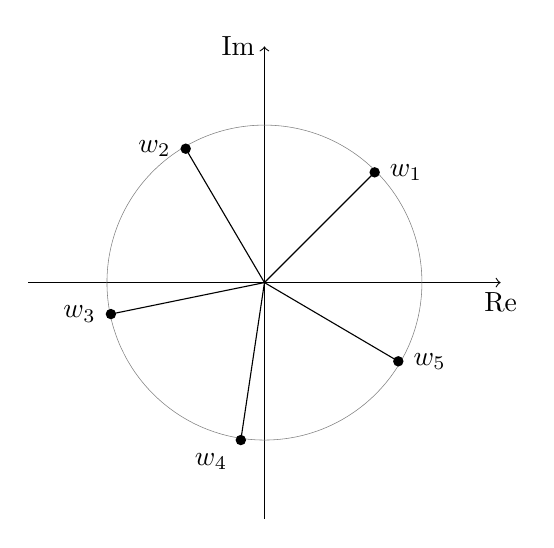
\begin{tikzpicture}
		\draw[->] (-3,0) -- (3,0) node[below] {Re};
		\draw[->] (0,-3) -- (0,3) node[left] {Im};
		\draw[help lines] (0,0) circle (2);
		
		\node[scale=0.4,circle,fill,label=right:{$w_1$}] at (1.4,1.4) {};
		\draw (0,0) -- (1.4,1.4);
		
		\node[scale=0.4,circle,fill,label=left:{$w_2$}] at (-1,1.7) {};
		\draw (0,0) -- (-1,1.7);
		
		\node[scale=0.4,circle,fill,label=left:{$w_3$}] at (-1.95,-0.4) {};
		\draw (0,0) -- (-1.95,-0.4);
		
		\node[scale=0.4,circle,fill,label=below left:{$w_4$}] at (-0.3,-2) {};
		\draw (0,0) -- (-0.3,-2);
		
		\node[scale=0.4,circle,fill,label=right:{$w_5$}] at (1.7,-1) {};
		\draw (0,0) -- (1.7,-1);
		\end{tikzpicture}
	\end{center}
	
		
	
\end{document}